% fig2_schema.pdf -- Tag schema 5 macro x 69 binary + 3 numeric (TikZ).
% Compile: PATH=$HOME/.TinyTeX/bin/x86_64-linux:$PATH xelatex _make_fig2_schema.tex
% Then rename _make_fig2_schema.pdf -> fig2_schema.pdf
\documentclass[border=2pt,tikz]{standalone}
\usepackage[T1]{fontenc}
\usepackage{lmodern}    % Latin Modern (vector at every size; consistent with Fig 1/6)
\usepackage{amsmath}
\usepackage{tikz}
\usetikzlibrary{positioning,calc,fit,backgrounds}

\begin{document}
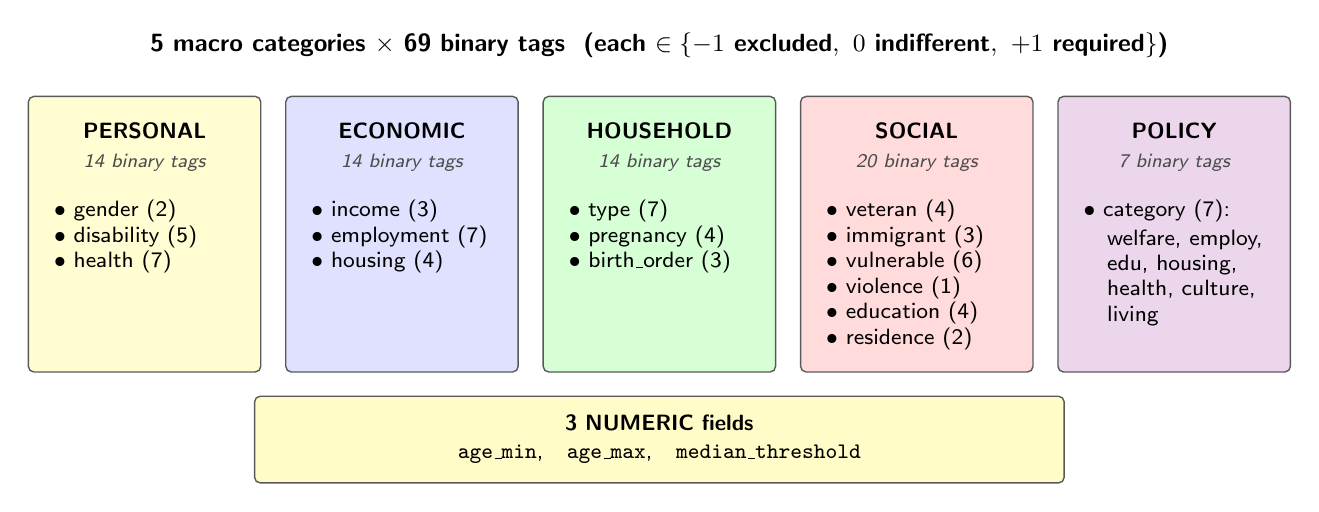
\begin{tikzpicture}[
  font=\sffamily,
  every node/.style={inner sep=2pt},
  groupbox/.style={
    rectangle, rounded corners=2pt,
    draw=black!65, line width=0.5pt,
    align=center,
    minimum height=3.5cm,
    text width=2.6cm,
    inner sep=5pt,
    font=\sffamily\fontsize{7.8}{9.4}\selectfont,
  },
  numbox/.style={
    rectangle, rounded corners=2pt,
    draw=black!65, line width=0.5pt,
    fill=yellow!22,
    align=center,
    text width=10.0cm, minimum height=1.10cm,
    inner sep=4pt,
    font=\sffamily\fontsize{8}{10}\selectfont,
  },
  hdr/.style={font=\sffamily\bfseries\fontsize{8.5}{10}\selectfont},
  cnt/.style={font=\sffamily\itshape\fontsize{7.2}{8.4}\selectfont, text=black!70},
  itm/.style={font=\sffamily\fontsize{7.6}{9.2}\selectfont},
]

% ----- 5 equal-width macro group boxes for visual balance -----
\def\gapH{0.30cm}

% PERSONAL
\node[groupbox, fill=yellow!18, anchor=west] (G1) at (0,0) {};
% ECONOMIC
\node[groupbox, fill=blue!12, right=\gapH of G1.east, anchor=west] (G2) {};
% HOUSEHOLD
\node[groupbox, fill=green!16, right=\gapH of G2.east, anchor=west] (G3) {};
% SOCIAL
\node[groupbox, fill=red!14, right=\gapH of G3.east, anchor=west] (G4) {};
% POLICY
\node[groupbox, fill=violet!16, right=\gapH of G4.east, anchor=west] (G5) {};

% ----- inside each box: header + count + bullet items -----
% PERSONAL (14)
\node[hdr] at ($(G1.north) + (0,-0.45)$) {PERSONAL};
\node[cnt] at ($(G1.north) + (0,-0.85)$) {14 binary tags};
\node[itm, anchor=north, align=left, text width=2.3cm]
  at ($(G1.north) + (0,-1.25)$)
  {$\bullet$\ gender (2)\\
   $\bullet$\ disability (5)\\
   $\bullet$\ health (7)};

% ECONOMIC (14)
\node[hdr] at ($(G2.north) + (0,-0.45)$) {ECONOMIC};
\node[cnt] at ($(G2.north) + (0,-0.85)$) {14 binary tags};
\node[itm, anchor=north, align=left, text width=2.3cm]
  at ($(G2.north) + (0,-1.25)$)
  {$\bullet$\ income (3)\\
   $\bullet$\ employment (7)\\
   $\bullet$\ housing (4)};

% HOUSEHOLD (14)
\node[hdr] at ($(G3.north) + (0,-0.45)$) {HOUSEHOLD};
\node[cnt] at ($(G3.north) + (0,-0.85)$) {14 binary tags};
\node[itm, anchor=north, align=left, text width=2.3cm]
  at ($(G3.north) + (0,-1.25)$)
  {$\bullet$\ type (7)\\
   $\bullet$\ pregnancy (4)\\
   $\bullet$\ birth\_order (3)};

% SOCIAL (20)
\node[hdr] at ($(G4.north) + (0,-0.45)$) {SOCIAL};
\node[cnt] at ($(G4.north) + (0,-0.85)$) {20 binary tags};
\node[itm, anchor=north, align=left, text width=2.3cm]
  at ($(G4.north) + (0,-1.25)$)
  {$\bullet$\ veteran (4)\\
   $\bullet$\ immigrant (3)\\
   $\bullet$\ vulnerable (6)\\
   $\bullet$\ violence (1)\\
   $\bullet$\ education (4)\\
   $\bullet$\ residence (2)};

% POLICY (7) -- horizontal comma-separated to avoid cramped vertical list
\node[hdr] at ($(G5.north) + (0,-0.45)$) {POLICY};
\node[cnt] at ($(G5.north) + (0,-0.85)$) {7 binary tags};
\node[itm, anchor=north, align=left, text width=2.3cm]
  at ($(G5.north) + (0,-1.25)$)
  {$\bullet$\ category (7):\\[1pt]
   \quad welfare, employ,\\
   \quad edu, housing,\\
   \quad health, culture,\\
   \quad living};

% ----- 3 NUMERIC strip below, centered horizontally with the 5 boxes -----
\node[numbox] (N) at ($(G1.south west)!0.5!(G5.south east) + (0,-0.85)$)
  {\textbf{3 NUMERIC fields}\\
   \texttt{age\_min},\quad \texttt{age\_max},\quad \texttt{median\_threshold}};

% ----- top legend / 3-state semantics -----
\node[anchor=south, font=\sffamily\bfseries\fontsize{8.6}{10}\selectfont]
  at ($(G1.north west)!0.5!(G5.north east) + (0,0.40)$)
  {5 macro categories $\times$ 69 binary tags
    \ (each $\in \{-1\ \text{excluded},\ 0\ \text{indifferent},\ +1\ \text{required}\}$)};

\end{tikzpicture}
\end{document}
